\documentclass{article}
\title{Automaten en Berekenbaarheid:\\opgave 1}
\author{Prof. B. Demoen (\url{Bart.Demoen@cs.kuleuven.be})\\ W. Van Onsem (\url{Willem.VanOnsem@cs.kuleuven.be})}
\date{5 november 2013}
\usepackage{tikz,../assignment-nl}
\usetikzlibrary{automata,arrows,decorations.pathmorphing,backgrounds,positioning,fit}
\newcommand{\lang}[1]{\textsc{#1}}
\begin{document}
\maketitle
\paragraph{Richtlijnen}

Je schrijft enkel op de gekleurde bladen die je gekregen hebt: op je
werkplek liggen geen andere bladen dan die gekleurde bladen en de
bladen van de cursustekst. De bladen van je cursustekst waarop
oplossingen van oefeningen of aanwijzingen tot oplossingen van
oefeningen staan, steek je ook weg. Je jas, je boekentas, je gsm
... leg je vooraan in het auditorium, zoals gebruikelijk bij een
examen. Bij het afgeven zorg je dat je naam op je bladen staat, en dat
je alles aan elkaar niet. Er zijn 4 vragen.

\begin{question}[Pompend lemma voor reguliere talen]
Indien de voorgestelde taal niet regulier is: bewijs dit aan de hand van het pompend lemma voor reguliere talen. Indien
de voorgestelde taal dit wel is: geeft een reguliere expressie of een eindige toestandsautomaat die de taal
beschrijft/beslist.
\begin{enumerate}
 \item De verzameling strings uit $\Sigma=\accl{a,b}$ zodat voor elke string $s\in\Sigma^\star$, $s\in L$ indien voor
elke prefix\footnote{Een prefix van $s$ is een substring van $s$ die begint bij het eerste karakter van $s$ en op een
willekeurige plaats $k$ eindigt.} van $s$ het aantal $a$'s en $b$'s in de string nooit meer dan 2 verschilt.
 \item $L=\accl{a^mc^nb^m|m,n\in\NN\mbox{ met $m> n$}}$
 \item $L=\accl{a^mb^n|m,n\in\NN\mbox{ met $m<n$ en $m<981$}}$.
 \item $L=\accl{wv^\star w|v\in\Sigma,w\in\Sigma^\star}$ voor een willekeurige eindige $\Sigma$ die uit
minstens twee elementen bestaat.
\end{enumerate}
\end{question}
\begin{answer}[Pompend lemma voor reguliere talen]
We beschouwen de verschillende talen.
\begin{enumerate}
 \item Regulier. Vermits de eigenschap voor iedere prefix geldt, kunnen we een transitie-eigenschap uitbuiten: een string maakt nog kans om geaccepteerd te worden indien in het verleden het verschil nooit meer dan twee bedroeg. We beschouwen dus 5 accepterende toestanden die het verschil van -2 tot 2 opslaan. Telkens wanneer een $a$ of $b$ wordt uitgelezen, gaan we naar een toestand die \'e\'entje hoger of lager is. Wanneer we een $a$ lezen bij $-2$ of een $b$ bij $2$ komen we in een ongeldige toestand terecht. Deze zal de overige karakters inlezen zonder in een accepterende eindtoestand te eindigen.\\
 \begin{center}
 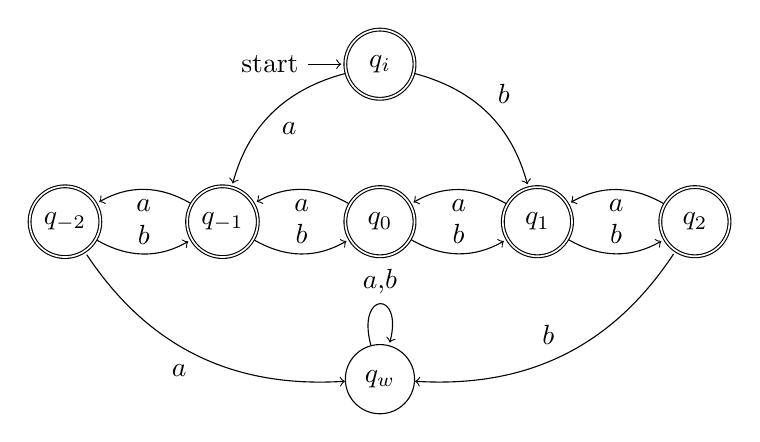
\begin{tikzpicture}[shorten >=1pt,node distance=2cm,on grid,auto]
 \node[state,initial,accepting]   (qi) {$q_i$};
 \node[state,accepting] (q0) [below=of qi] {$q_0$};
 \node[state,accepting] (q9) [left=of q0] {$q_{-1}$};
 \node[state,accepting] (q8) [left=of q9] {$q_{-2}$};
 \node[state,accepting] (q1) [right=of q0] {$q_1$};
 \node[state,accepting] (q2) [right=of q1] {$q_2$};
 \node[state]           (qw) [below=of q0] {$q_w$};
 \path[->] (qi) edge [bend right] node {$a$} (q9) edge [bend left] node {$b$} (q1);
 \foreach \i/\j in {8/9,9/0,0/1,1/2} {
   \path[->] (q\j) edge [bend right] node {$a$} (q\i);
   \path[->] (q\i) edge [bend right] node {$b$} (q\j);
 }
 \path[<-] (qw) edge [bend left] node {$a$} (q8) edge [bend right] node {$b$} (q2);
 \path[->] (qw) edge [loop above] node {$a$,$b$} ();
 \end{tikzpicture}
 \end{center}
 \item Niet-regulier.
 \item Regulier. We construeren eerst een reguliere expressie aan de hand van een parameter $i$:
 \begin{equation}
  a^ib^ib^\star
 \end{equation}
 Vervolgens is $L$ gelijk aan een eindige unie:
 \begin{equation}
  \cup_{i=0}^980 a^ib^ib^\star
 \end{equation}
Concreet ziet de reguliere expressie er dus als volgt uit:
\begin{equation}
 b^\star\ |\ abb^\star\ |\ aabbb^\star\ |\ aaabbbb^\star\ |\ \cdots\ |\ \underbrace{aaaaa\cdots a}_{980\mbox{\small{ keer}}}\underbrace{bbbbb\cdots b}_{980\mbox{\small{ keer}}}b^\star
\end{equation}

 \item Niet-regulier. Stel dat $a$ en $b$ twee elementen uit $\Sigma$ zijn\footnote{Hoe de symbolen eruit zien maakt niet uit, evenmin dat er nog andere symbolen betrokken zijn.}. In dat geval beschouwen we de string $s=a^dbc^d$. Deze string $\abs{s}>d$
\end{enumerate}
\end{answer}
\begin{question}[Algebra van talen]
Niet alle talen behoren tot \emph{RegLan}, denk bijvoorbeeld aan $\lang{AGelijkB}=\accl{a^nb^n|n\in\NN}$. Stel dat $L_1$
en $L_2$ verschillende niet-reguliere talen zijn; en $L_3$ en $L_4$ verschillende oneindige reguliere talen niet gelijk
aan $\Sigma^*$ met $\Sigma$ het alfabet van de talen in kwestie. Zijn volgende talen dan regulier, niet-regulier of
hangt dit af van de talen in kwestie. Bewijs of geef tegenvoorbeelden.
\begin{enumerate}
 \item $L_1\cap L_3$.
 \item $L_1\cup L_3$.
 \item $L_1\cup L_2$.
 \item $\overline{L_1}\cup L_3$.
\end{enumerate}
\end{question}

\begin{question}[Pompend lemma voor contextvrije talen]
Indien de voorgestelde taal niet context-vrij is: bewijs dit aan de hand van het pompend lemma voor contextvrije talen.
Indien de voorgestelde taal dit wel is: geeft een reguliere expressie, een eindige toestandsautomaat, een contextvrije
grammatica of een push-down automaat die de taal beschrijft/beslist.
\begin{enumerate}
 \item $L=\accl{a^mb^nc^{n+m}|m,n\in\NN}$
 \item $L=\accl{a^mb^nc^md^n|m,n\in\NN}$
 \item $L_R=\accl{wv\hat{w}|w\in\Sigma^*\wedge v\in R}$ voor een willekeurige eindige $\Sigma$ die uit minstens twee
elementen bestaat en $R$ een reguliere taal over $\Sigma$.
\end{enumerate}
\end{question}
\begin{answer}[Pompend lemma voor contextvrije talen]
We beschouwen de verschillende talen.
\begin{enumerate}
 \item Context-vrij.
 \item Niet context-vrij.
 \item Context-vrij.
\end{enumerate}
\end{answer}
\begin{question}[Myhill-Nerode relaties]
Gegeven de volgende twee partities:
\begin{eqnarray}
P_1=\accl{\accl{a,b},\accl{c},\accl{d},\accl{e,f,g},\accl{h} }\\
P_2=\accl{\accl{a,e},\accl{b,c},\accl{d,h},\accl{f,g} }
\end{eqnarray}
Bepaal het supremum van de twee partities volgens de theorie in de cursus (sectie 13.3).
\end{question}
\begin{answer}[Myhill-Nerode relaties]
Het supremum is gedefinieerd als de \emph{fijnste relatie die grover is dan de originele relaties}. De resulterende relatie is dan:
\begin{equation}
P=\accl{\accl{a,b,c,e,f,g},\accl{d,h} }
\end{equation}
\end{answer}
\end{document}